\normaltrue \difficilefalse \tdifficilefalse
\correctionfalse

%\UPSTIidClasse{11} % 11 sup, 12 spé
%\newcommand{\UPSTIidClasse}{11}

\exer{Sécateur $\star$ \label{G2:01:2004}}
\setcounter{question}{0}\marginnote{\xpComp{PPM}{02}}%\UPSTIcompetence[2]{G2-01}
\index{Compétence G2-01}\index{Compétence PPM-02}

\ifcorrection
\else
\marginnote{\textbf{Pas de corrigé pour cet exercice.}}
\fi


\ifprof 
\else
Soit la pièce suivante.
\begin{center}
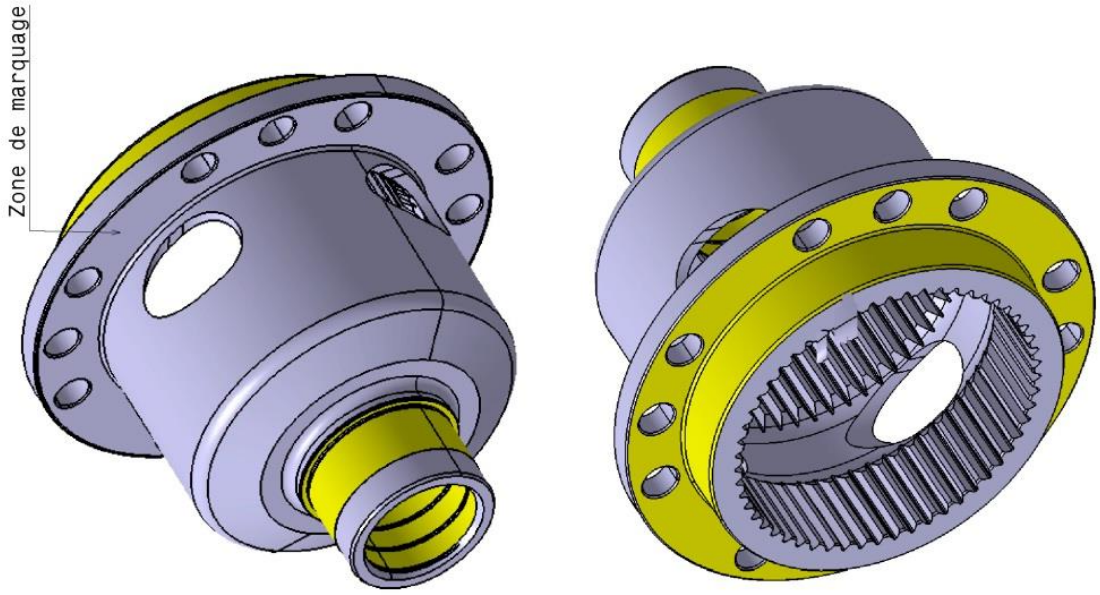
\includegraphics[width=.8\linewidth]{fig_01}
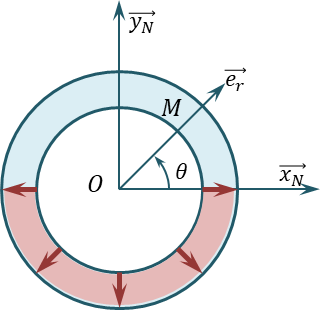
\includegraphics[width=.8\linewidth]{fig_02}
\end{center}
 \fi
 
\question{Proposer une gamme de fabrication, de l'élaboration du brut à la finition.}
\ifprof
\begin{marginfigure}
%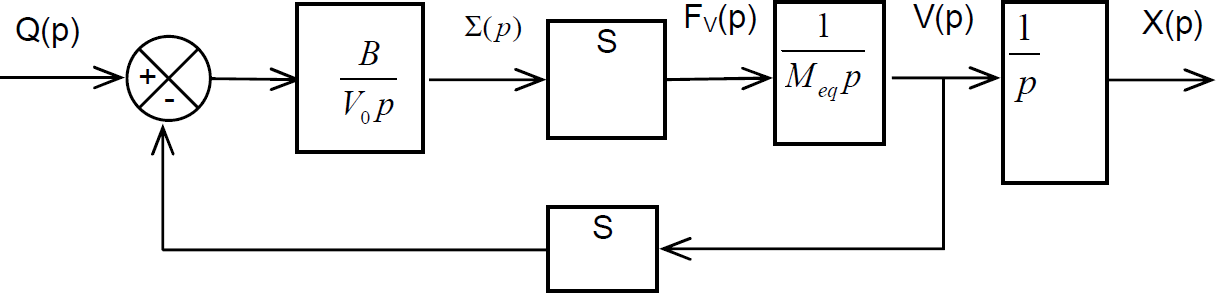
\includegraphics[width=\linewidth]{cor_01}
\end{marginfigure}

\else 
\fi

\question{La pièce a été réalisée en acier allié. Justifier ce choix.}

\question{La fatigue est un des critères de dimensionnement de cette pièce. Décrire cet essai.}


\ifprof
\else

\marginnote{Corrigé voir \ref{G2:01:2004}.}

\fi